% This is samplepaper.tex, a sample chapter demonstrating the
% LLNCS macro package for Springer Computer Science proceedings;
% Version 2.20 of 2017/10/04
%
\documentclass[runningheads]{llncs}
%
\usepackage{graphicx}
%\usepackage[utf8]{inputenc}
%\usepackage[english]{babel}
\usepackage{amsthm}
\usepackage{algorithm}
% Used for displaying a sample figure. If possible, figure files should
\usepackage{algpseudocode}
%\usepackage[linesnumbered,ruled,vlined]{algorithm2e}

% be included in EPS format.
%
% If you use the hyperref package, please uncomment the following line
% to display URLs in blue roman font according to Springer's eBook style:
% \renewcommand\UrlFont{\color{blue}\rmfamily}

\newtheorem*{myProbStatement}{Problem Statement}

\begin{document}
%
\title{Fake-and-Real News Detection and Analysis}
%
%\titlerunning{Abbreviated paper title}
% If the paper title is too long for the running head, you can set
% an abbreviated paper title here
%
\author{
Medha Gulati\,
Avishi Goyal\,
Shivangi Mishra\and
Pooja Garg\
}
%
\authorrunning{BI-Team-9}
% First names are abbreviated in the running head.
% If there are more than two authors, 'et al.' is used.
%
\institute{Indira Gandhi Delhi Technical University for Women, Delhi, India\newline
\email{\{ahdemitalug, goyalavishi, s.mishra9703, poojagarg144\}@gmail.com}}
%
\maketitle              % typeset the header of the contribution
%
\begin{abstract}
Is it possible to differentiate the real news from fake news? Can we tell that which media websites are stating the truth?
The news legitimacy is becoming an issue that needs an immediate attention since it affects our social lives and the environment at our workplaces. The fact that social media is used to keep oneself updated by a million of users all over the globe, its quite easy for the fake news articles to be circulated exponentially that creates a false alarm among the audience and creates negative impacts among them in the shortest time frame.  
We here, try to solve this issue of fake news through the concepts of machine learning by predicting if the content of information is real or fake.

\keywords{Fake News \and Real News \and Natural Language Processing \and Machine Learning.}
\end{abstract}
%
%
%
\section{Introduction}
Fake news or misleading information are being updated on several social media platforms nowadays. The sources of such news have always been the social media platforms that are used all over the globe by a variety of audiences as a commonplace to search and explore the articles that concern their areas of interests and work. With the rapid growth of this social media surfing, one side it creates an opportunity for every person to live his/her liberty and freedom by allowing them to portrait their views and agendas but on the other hand it allows breeding to a number of people who misuse this social media stage to create and publish false news. 
The results of such habits have changed the way people on receiving end view media of modern era. Receivers of news tend to judge the authenticity of various articles depending upon their favouritism of that particular news.
This has become an issue of great debate that the social media which was once used to reach the public to create awareness and to bind the world at one place has itself become the most desired platform to spread rumours and mislead people and hence, affecting the way they react to different situtions.


% \subsubsection{Sample Heading (Third Level)} You can also have sub-sub-section, optionally.


% \noindent Displayed equations are centered and set on a separate. Note that equation numbering is done automatically. Eg \ref{eq-add} explains addition of $x$ and $y$ into $z$.

% \begin{equation}
% \label{eq-add}
% x + \frac{y}{2} = z^{e}
% \end{equation}

\subsection{Problem Statement}
 \newline
% You can include a new definition block as below.

Given a news article with a headline and some text. The problem is to detect whether the news article is fake or real.

\subsection{Objective}
 \newline
 
In this section, objective of the study is presented-
\newline
\newline
 \emph{Data Acquisition:} The aim is to collect a data set of fake news and real news. The data set to be collected can be both in collective and atomic form. We aim to get the data set as big as possible to check the proper working of our algorithm.
\newline 
\newline
 \emph{Fake and Real News Detector:} The aim is to train our machine learning modals to learn differences in pattern of real and fake news. 
Multiple modals are trained on different feature sets related to news title, body and subject. Trained modal are tested using test data sets and corresponding accuracy is noted. If the modals show desired accuracy, then the algorithm is approved to be used as the Fake and Real News Detector. 
\newline
\newline
 \emph{Deployment of code using Whatsapp business API:} As a final step, deploy trained modals on whatsapp business API to check the legitimacy of the news being published on these platforms.

\subsection{Scope and Limitation}
\emph{Limitation:}
Since these trained modals depends on writing style, So by changing the writing style, results may vary.
\newline
\newline
\emph{Scope:}
Since almost everyone now-a-days are using whatsapp. through this whatsapp can used as the news delivering platform.

\section{Related Work}
In [1] and [2], the authors distinguish fake from genuine news and show sources and audiences of fake news. These articles classify the sources of news (like social media) as authentic or not. In [3]& [4] , the conflicting viewpoints of observing "likes" and "comments" can be seen. They consider only metadata for the classification tasks. 
We consider text classification of news for determining if it is fake or not. The text classification along with sentiment analysis is a better way of classifying news.
\section{Methodology}

Our dataset contains two kinds of news, that are fake and real news. We are trying to classify them into the above two categories and further analyze them.


\subsection{Dataset Description}
The data was collected from Kaggle.
Kaggle is Google LLC's affiliate that allows data science learners and analysts to explore various data sets on a web-based platform of data science. It allows various practitioners of machine learning to work as a community and helps them in solving the new and upcoming challenges of data science.
Kaggle was started in the year 2010 and created an uproar among all the data scientists and machine learning enthusiasts as it provides an opportunity to get a hold of various competitions in the field of artificial intelligence over a cloud-based network. 

Also explain the method adopted for collection of this data, if it is mentioned in source URL.

Table \ref{tbl:dataset} is an example describing the dataset through counts of some key entities involved in the dataset.
\begin{table}
\centering
\begin{tabular}{|l|c|}
\hline
\textbf{Details} &  \textbf{Count}\\
\hline
Number of Fake News & 17,903 \\
\hline
Number of Real News & 20,826\\
\hline
\end{tabular}
\caption{Details of the dataset.}
\label{tbl:dataset}
\end{table}

Every dataset also comprises of data attributes. Table \ref{tbl:dataset-attributes} describes attributes of data.
For supervised learning, the attribute(s) \textit{Fake, Real} would be considered as labels. 

\begin{table}
\centering
\begin{tabular}{|l|c|}
\hline
\textbf{Data Attributes} &  \textbf{Brief Explanation}\\
\hline
Title & Title of the article \\
\hline
Text & Body of the article \\
\hline
Date & Date the article was posted on\\
\hline
\end{tabular}
\caption{Details of Data Attributes.}
\label{tbl:dataset-attributes}
\end{table}

\subsection{Data Pre-processing}
Data is available in the form of fake.csv and real.csv files holding information for real and fake data separately. 
Following steps were involved in preprocessing-

\subsubsection{Basic text pre-processing}
\newline
\newline
\begin{enumerate}
\item \textbf{\emph{Removing Duplicates.}}
These files were combined to form one dataset. The rows containing duplicate data were removed. 
\newline
\newline
\item \textbf{\emph{Removing Punctaution.}}
All punctuation marks are removed, since they do not contain any relevant information.
\newline
\newline
\item \textbf{\emph{Tokenization}}
Data is tokenized i.e. body of the text/paragraph is splitted into sentences and words. These words are known as tokens.
\item \textbf{\emph{Normalization. }} 
Data is converted to same format, to normalize data.
Eg- Convert whole data to lower case or upper case.
\newline
\newline
\item \textbf{\emph{Remove stopwords. }}
Stopwords are the most commonly used token words. Eg- 'the','an',etc. They are ignored during processing data as they do not give meaning to a sentence. They are only used to give sentence a structure.
\newline
\newline
\item \textbf{\emph{Stemming and Lemmatization. }}
Stemming and lemmatization are process of reducing words with same meaning into one. These are also normalization techniques only. Purpose is to minimize text ambiguity.
\newline
\newline
\end{enumerate}

\subsubsection{Basic Feature Extraction}
\begin{enumerate}
\item \textbf{\emph{Number of words.}}
\begin{figure}
\centering
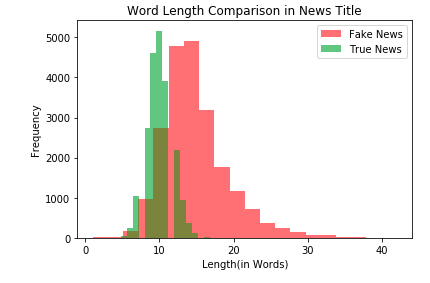
\includegraphics[width=8cm]{wordLenTitle.png}
\caption{Fig shows the graph between the length distribution of headlines/title for fake and real news It is observed that the headlines/title of fake news articles have more length as compared to the title of real news articles} \label{fig1}
\end{figure}

\begin{figure}
\centering
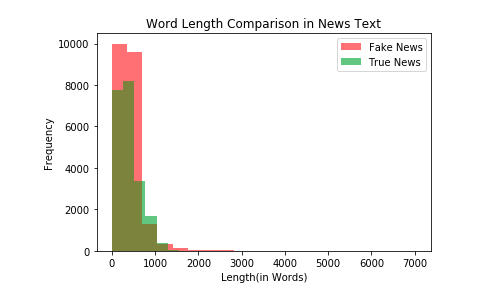
\includegraphics[width=8cm]{wordLenText.png}
\caption{It shows the graph between the length distribution of text for fake and real news. whereas it is not the same in the case of length values of text, i.e. the text of real news articles have smaller length values as compared to the fake news articles.} \label{fig2}
\end{figure}
\newpage
\item \textbf{\emph{Number of Characters.}}
\begin{figure}
\centering
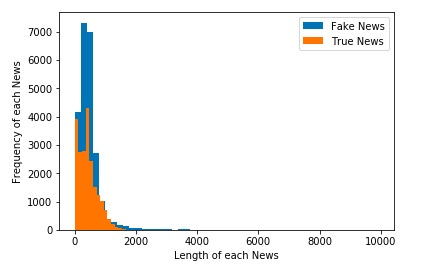
\includegraphics[width=8cm]{characterCountText.jpeg}
\caption{It shows the graph between the length distribution of characters in text for fake and real news.} \label{fig2}
\end{figure}
\newpage
\item \textbf{\emph{Number of stopwords}}
\begin{figure}
\centering
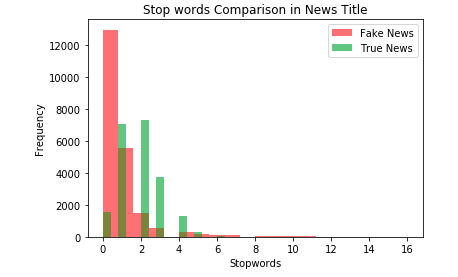
\includegraphics[width=7cm]{stopTitle.png}
\caption{It shows the comparison in frequency of Stopwords in the headline of fake and real news} \label{fig3}
\end{figure}
\begin{figure}
\centering
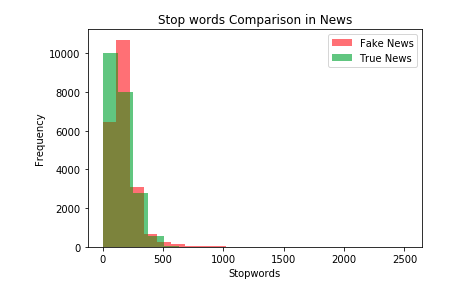
\includegraphics[width=8cm]{stopText.png}
\caption{It shows the comparison between the text of real and fake news. It is observed that the frequency of Stopwords is high in the case of fake news when compared according to headlines but when comparing the text of the article, both fake and real news have almost the same frequency of Stopwords.} \label{fig4}
\end{figure}
\end{enumerate}
\newpage
\begin{enumerate}
\subsubsection{Advance Text Preprocessing}

\item \textbf{\emph{Ngrams.}}
Ngrams refers to the sequences of n words. for e.g (BI report) is bigram or a 2-gram, (Team 9 Report) is trigram or 3-gram. Ngrams are used for various purposes like auto completion, spell check, etc.
\newline
\newline
\item \textbf{\emph{Bag of words.}}
Bag of words is used for pre-processing purposes to actually create a bag that consists of all the words used in text body along with the count of their occurrences. It helps to analyze the words of the whole text atomically and also helps to keep a check on the most frequent words.
\newline
\newline
\item \textbf{\emph{Sentiment Analysis.}}
Sentimental Analysis is a technique to check the polarity of any sentiment present in an article. During our research we found that fake news has more catchy sentences to draw the attention of their viewers. We tried to use sentiment analysis on the text of news articles and found the same results. We collected the emotion words present in the text of the article and compared then with the words present in emotions.txt and found that the fake news articles have more amount of negative emotions as compared to true news articles.
\begin{figure}
\centering
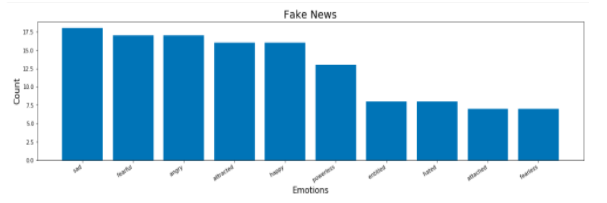
\includegraphics[width=10cm]{fake.png}
\caption{Fig above displays the count of different emotions (embarrassed, fearful, demoralized, ecstatic, bored obsessed, attracted, cheated, etc.) in case of fake and real news. It is observed that the fake news consists of more dominant negative emotions (hatred, sad , fearful , anger etc) while the true news consists more of positive emotions or neutral emotions (happy, attracted etc ). This comparison can help us separate fake news more easily from true news.} \label{fig3}
\end{figure}
\begin{figure}
\centering
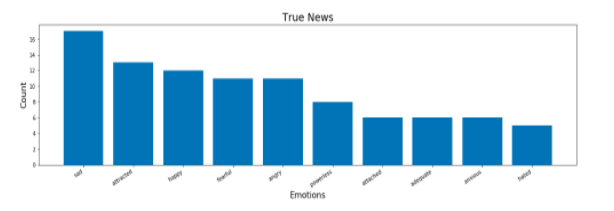
\includegraphics[width=10cm]{real.png}
\caption{Fig. above displays the count of different emotions (embarrassed, fearful, demoralized, ecstatic, bored obsessed, attracted, cheated, etc.) in case of fake and real news. It is observed that the fake news consists of more dominant negative emotions (hatred, sad , fearful , anger etc) while the true news consists more of positive emotions or neutral emotions (happy, attracted etc ). This comparison can help us separate fake news more easily from true news.} \label{fig4}
\end{figure}
\newpage
\item \textbf{\emph{Language Analysis.}}
The language checker library to check the mistakes occurred in the grammar of the news articles.
In this the input  of the news articles and the output is a set of all the grammatical rules that are incorrectly implemented. The number of mistakes in grammar are found using the matches function.
A comparison is done between the number of mistakes in real and fake news. Thus we see that there are more grammatical errors in fake news as compared to true news.

\begin{figure}
\centering
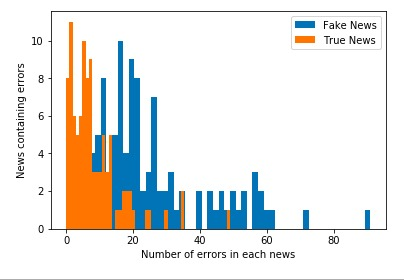
\includegraphics[width=10cm]{lang.jpeg}
\caption{Fig. above displays the number of errors in the language of each true news and each fake news} \label{fig4}
\end{figure}
\newpage
\item \textbf{\emph{Vectorization. }}
Vectorization is among the most popular methodology of Natural Language Processing, it is used to map words and phrases into real numbers to find the similarities in semantics of vocabulary.
\newline
\newline
\t Two different type of vectorizer used are:
\newline
1. Count Vectorizer: Works on frequency of occurrence of words and phrases. Tokens are counted and a sparse matrix is build for document and tokens.  
\newline
\newline
2. TF-IDF: Here frequency of occurrence of words and phrases are seen but also how important a token is noted. Tokens with maximum frequency are most important.
\newline
\newline
The data set is then split into a training set and testing set as 67\% and 33\% of the data respectively.
\end{enumerate}
\section{Proposed Approach}
This section explains the details of how the above mention objective is achieved. Multinomial Naive Bayes and Random Forest algorithms are used to make the predictions. These two approaches work well with big data sets and provide the predictions with high accuracy. Data set learning and training phase of these algorithms is fast and hence are the first choice of eager learners. Following is the flow chart, diagrammatically representing the steps involved: 

\begin{figure}
\centering
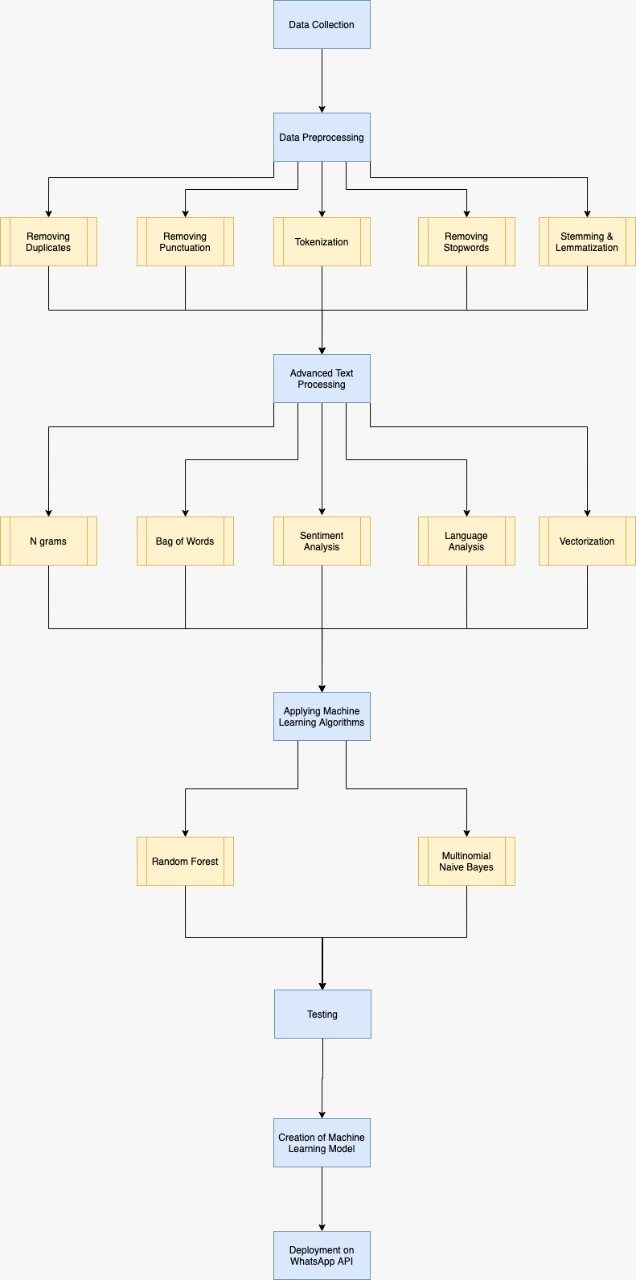
\includegraphics[width=10cm]{proposedmethodology.jpeg}
\caption{Proposed Methodology} \label{fig1}
\end{figure}


\newpage
\subsection{Fake and Real news Classifier}
After data cleaning and preparation, to train the fake and real classifier various different machine learning algorithms are used. A good classifier is the one which classifies the text type with great precision. The inputs of fake and real news classifier are the title, text and date of new instances of news. These inputs are processed according to the algorithms below and provides the output as real/fake and hence classifies the news articles.
\newline
\newline
\textbf{Input:}
\newline
\begin{itemize}
  \item Dataset containing news (say d)
  \item A fixed set of classes c = \{True news,Fake news\}
  \item A training set m, labelled document \[(d_1,c_1),(d_2,c_2), ..... , (d_n,c_n)\]
\end{itemize}
\textbf{Output:}
\newline
\begin{itemize}
  \item a learned classifier \[y: d -\rangle c\]
  \item accuracy of the classifier
\end{itemize}

\subsubsection{Multinomial Naive Bayes Classifier Algorithm}

The algorithm will estimate the conditional probability of a particular word given in a class as in relation frequency of term(t) which can occur multiple number of times in the training documents.It is mostly used in (NLP) natural language processing problems.The multinomial distribution normally requires integral count for features. We have used tf-idf vectorisor hence we have used Multinomial NB for classification.


\[{\displaystyle p(\mathbf {x} \mid C_{k})={\frac {(\sum _{i}x_{i})!}{\prod _{i}x_{i}!}}\prod _{i}{p_{ki}}^{x_{i}}}\]

\newline
where p(i) , p(j) is the probability that event i occurs (or K such multinomials in the multi-class case. Where x(i) counting the number of times event i was observed in a particular instance.

\subsubsection{Random Forest}
Random forest is a supervised learning algorithm used for the classification of data. As the name suggests, it deals with the methodology where a forest of trees is created (the larger the number of trees, the better we get the result) by choosing a random number 'r'  to divide the features of data set or to divide the training data set into r units to create decision tress. These large number of individual decision trees operate as an ensemble. The prediction values of these individual trees are stored. The prediction value that is encountered the maximum number of times is treated as the final output of algorithm.




% \begin{algorithm} % enter the algorithm environment
% \caption{Bag of Words Algorithm} % explain in 1-2 sentences about the algorithm
% \label{algo1}
% \begin{algorithmic}
% \Procedure{BagOfWords}{}
% \State Initialize feature vector bg feature= [0, 0, ....0]
% \For{token in text.tokenize()} 
% \If{token in dict}
% \State token idx=getindex(dict, token)
% \State bg feature[token idx]++
% \Else 
% \State continue
% \EndIf
% \EndFor
% \State \Return bg feature
% \EndProcedure
% \end{algorithmic}
% \end{algorithm}
%

\section{Results}
\newline
\newline
According to the graphical and tabular representation given below, it is observed that Multinomial Naive Bayes Classifier is a better approach than Random Forest Learning to classify news articles as fake or real as it provides predictions with great accuracy.
Multinomial Naive Bayes provides fast computations during learning stage and as soon as the model is learnt, it need not re-evaluate the training data set for making predictions. It also provides fast outputs for new instances.

\begin{table}[h!]
  \begin{center}
    \caption{Accuracy}
    \label{tab:table1}
    \begin{tabular}{l|c|r} % <-- Alignments: 1st column left, 2nd middle and 3rd right, with vertical lines in between
      \hline
      
      
      \textbf{Train-Test Ratio} & \textbf{Random Forest} & 
      
      \textbf{Multinomial Naive Bayes}\\
      
      \hline
      8:2 & 91.7483 & 94.9665\\
      \hline
      6:4 & 90.7182 & 94.3652\\
      \hline
      5:5 & 90.9082 & 94.2536\\
      \hline
      3:7 & 88.6474 & 93.3978\\
      \hline
      1:9 & 86.3025 & 91.9844\\
      \hline
      
    \end{tabular}
  \end{center}
\end{table}

\begin{figure}
\centering
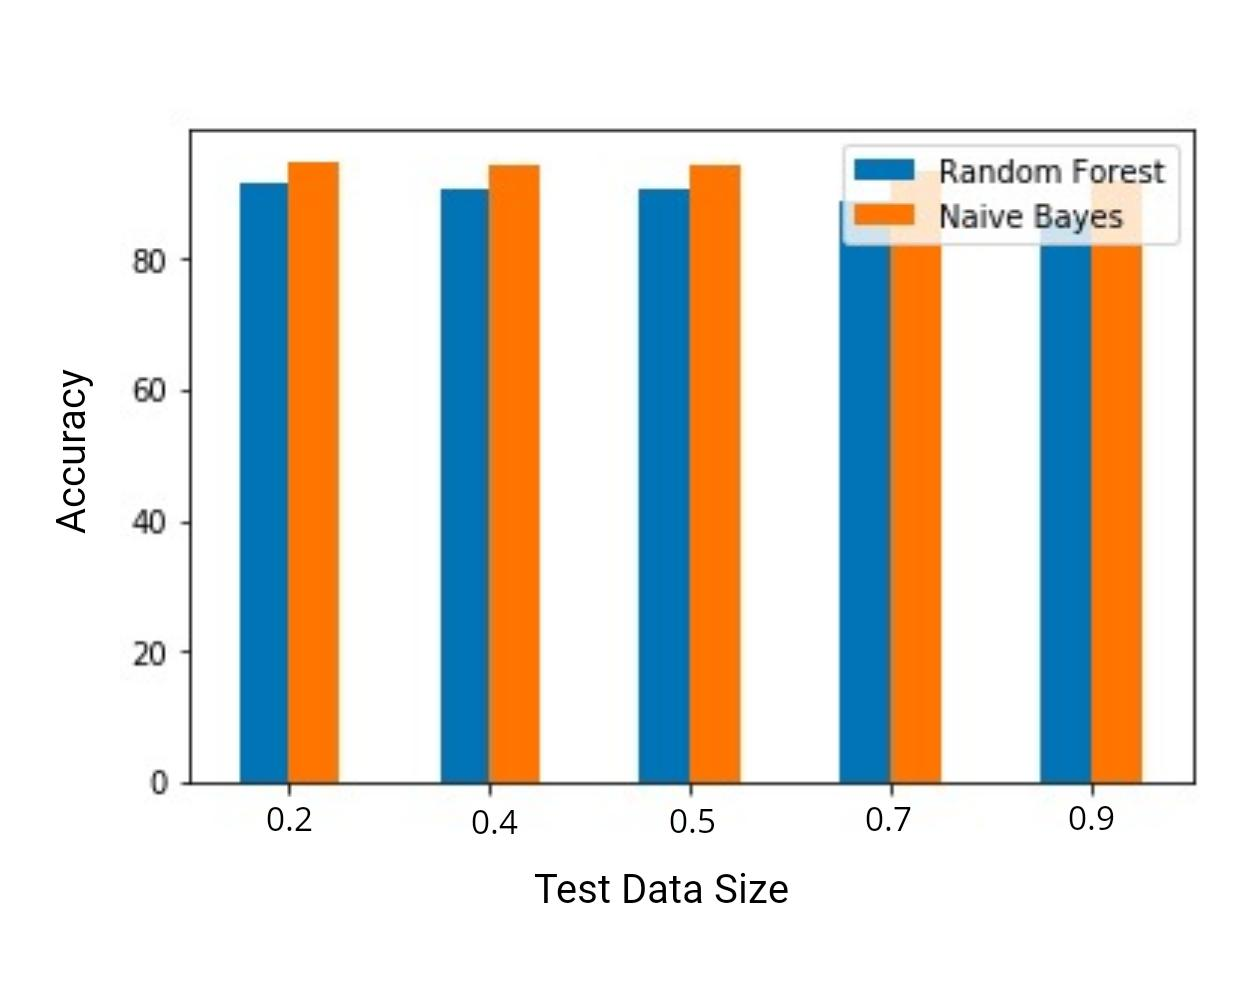
\includegraphics[width=10cm]{result.jpeg}
\caption{The above graph is comparing the accuracy of Random Forest and Naive Bayes algorithm in different train-test data proportions. } \label{fig9}
\end{figure}
\newline

\section{Future Work and Conclusion}
\subsection{Future works}
In the future , work can be performed on sentence structure, grammar, typos as features to improve the algorithm. We can also consider the metadata of the news article(like the website it was published on) as a secondary feature to improve the results. Lastly, an automated system for detection of fake news is also the need of the hour. Given the news text, the portal/website must be able to determine whether the news article is fake or real news in real time.

\subsubsection{Whatsapp as a news platform}
Since most the people today own a smartphone and uses whatsapp as a communication platform to things with the people they know. Using the above classifier and whatsapp business api, a new news sharing platform can be formed with the feature to validate news. Since people are more comfortable using whatsapp than any website.

\subsection{Conclusion}
According to the above research and analysis, it can be concluded that it is really important to classify the news as real/fake as the authenticity of news plays an important role on how the audience react to it. Misinformation can affect social and work lives of each person so it becomes a necessity to give reactions only to real news whereas the fake news should be ignored. 
\newline

\section{References}
[1] H. Allcott and M. Gentzkow, “Social Media and Fake News in the 2016 Election,” Journal of Economic Perspectives, vol. 31, no. 2, pp. 211–236, 2017. \newline\newline
[2] V. L. Rubin, Y. Chen, and N. J. Conroy, “Deception detection for news: Three types of fakes,” Proc. Assoc. Info. Sci. Tech., vol. 52, no. 1, pp. 1–4, 2015.\newline\newline
[3] Zhiwei Jin, Juan Cao, Yongdong Zhang, and Jiebo Luo, “News Verification by Exploiting Conflicting Social Viewpoints in Microblogs,” Proceedings of the Thirtieth AAAI Conference on Artificial Intelligence, pp. 2972–2978, 2016.\newline\newline
[4] W. Y. Wang, "Liar, Liar Pants on Fire": A New Benchmark Dataset for Fake News Detection. Available: http://arxiv.org/pdf/1705.00648. \newline \newline

\newpage

\bibliographystyle{splncs04}
%

\end{document}
